\documentclass[a4]{article}
\usepackage{gnuplottex}
\usepackage{csvsimple}
\usepackage{subcaption}
\usepackage{amsmath}
\usepackage{indentfirst}
\usepackage{graphicx}
\usepackage{float}
\usepackage{epstopdf}

\title{COMP26120 Lab 3 Report}
\author{XINYU LI}
\begin{document}
\maketitle
\tableofcontents
\newpage

\section{Experiment 1: Hash Set}

\subsection{Hypothesis}
Any string that is to be inserted into the hash table as an input value will have a unique hash value after being hashed. The complexity of both insert and find operation will be O(1).

With the linear probing, each string to be hashed will be inserted into one of the empty slots of the hash table with equal probability. Actually, the complexity will be between O(1) and O(n). In the worst case, each rehash will performance n constant time insertions or finds, so the complexity will be O(n). However, in fact, if a suitable initial hash table size is used, each insert or find will be collision-free, so the complexity will be O(1).

$$ h(k) = (sum^3) \ mod \ N $$
In this formula, k is a string, N is the length of hashset, sum is calculated by:
$$ sum = \sum^{N}_{i=0}(ord(k)^3) $$


\subsection{Design}
The original dataset I used was a seven-letter string generated randomly by a script. The size of the dataset varies with the size of the hash table used for testing. As all strings are randomly generated, the number must fit and satisfy the test requirements.

All input strings are made up of letters and do not contain any special symbols, which is more in line with the requirements of a dictionary. Although overall random letters without logic are less likely than words with actual meaning, they also reduce the chances of randomly generated input having properties that are not typical of the average case.

The script for generating and testing is python/experiment1.ipynb.

The script first generates a 7-letter random string, and the second generates a list of hash table sizes ranging from 500 to 100000, with an interval of 200. The time is recorded before and after the insert and find are performed to check the time taken for the whole operation and to facilitate subsequent recording. I created a dataframe with five columns containing set\_size, average\_insert, average\_find, collision\_rate, and time. The set\_size contains each size of the hash table, which was created before. This script calls the python/hashset.py to facilitate the recording of the data recorded in it into a dataframe for export to a csv file and for charting. The average\_insert, average\_find and collision\_rate are calculated in the hashset.py file, which is called and written to the dataframe in the script.

For each test, the script will add the generated random string to the word list and then call the hashset file, using the insert function and the find function to perform both operations. The script records the total time taken for each operation, the average number of inserts, the average number of finds, and the collision rate. Finally, the script will output the relationship between the size of the dataset and the above four data by generating scatter plots.

\subsection{Results}
The results show in the end part of python/experiment1.py.
\begin{figure}[H]
    \begin{minipage}{0.5\textwidth}        
    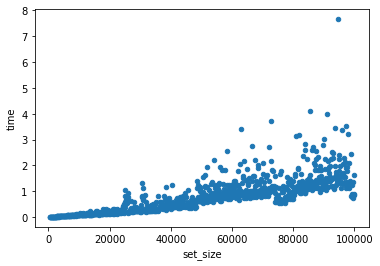
\includegraphics[width=0.95\textwidth]{hashset1.png}
    \caption{Time - Size}
    \end{minipage}
    \begin{minipage}{0.5\textwidth}        
    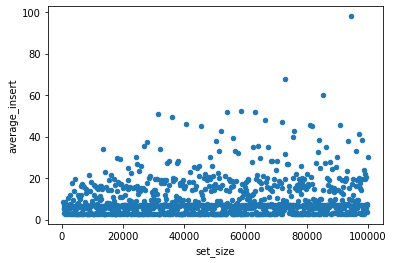
\includegraphics[width=0.95\textwidth]{hashset2.png}
    \caption{Average\_insert - Size}
    \end{minipage}
    \begin{minipage}{0.5\textwidth}        
    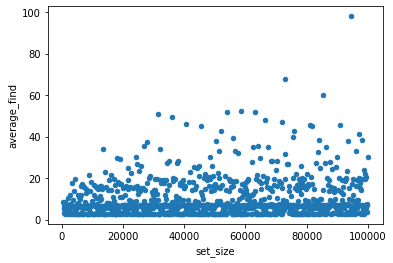
\includegraphics[width=0.95\textwidth]{hashset3.png}
    \caption{Average\_find - Size}
    \end{minipage}
    \begin{minipage}{0.5\textwidth}        
    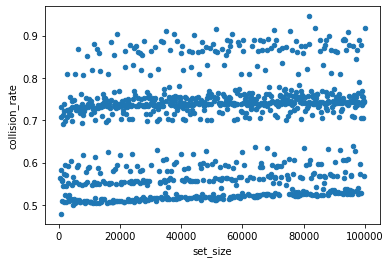
\includegraphics[width=0.95\textwidth]{hashset4.png}
    \caption{Collision\_rate - Size}
    \end{minipage}
\end{figure}
\noindent Average\_insert: the average number of data insertions during addressing.

\noindent Average\_find: the average number of data finds during addressing.

\noindent Collision\_rate: total number of collisions divided by hashset size.

\subsection{Discussion}
When using linear probing, the relationship between dataset size and total time per operation, the average number of inserts, the average number of finds and the collision rate are shown in the four graphs above.

From figure 1, it shows the relationship between time and size, with an overall trend of increasing time as size increases. It is worth noting that there are very few data that do not correspond to the overall trend. Due to the volume of data, deviations should be allowed.

From figure 2 and figure 3, they show the relationships between average insertions/finds and size. As the hashset size increases, their trend does not change significantly and most of the data is concentrated in the uniform interval, so the complexity is O(1).

From figure 4, it shows the relationship between collision rate and size. The collision rate is the total number of collisions divided by hashset size, and in this experiment, the collision rates of all the test data in the test set are concentrated in the interval 0.5-0.9, which reflects that the hash algorithm used is relatively good.

\subsection{Conclusion}
The hypothesis that the complexity of both the insertion and find operations will be O(1) is satisfied.

\newpage
\section{Experiment 2: Binary Search Tree}

\subsection{Hypothesis}
Any string that is to be inserted into the binary search tree as an input value will have a unique position as a node. The complexity of both insert and find operation will be O(logn).

In fact, for binary search trees, there are two kinds of cases, average case and worst case, which do not have the same complexity. For binary search trees with height balance property, the average case has O(logn) complexity, but for unbalanced binary search trees, the worst-case complexity will be O(n).

\subsection{Design}
The original dataset I used was a seven-letter string generated randomly by a script. The size of the dataset varies with the size/height of the binary search tree used for testing. As all strings are randomly generated, the number must fit and satisfy the test requirements.

All input strings are made up of letters and do not contain any special symbols, which is more in line with the requirements of a dictionary. Although overall random letters without logic are less likely than words with actual meaning, they also reduce the chances of randomly generated input having properties that are not typical of the average case.

The script for generating and testing is python/experiment2.ipynb.

The script first generates a 7-letter random string, and the second generates a list of binary search tree sizes ranging from 500 to 100000, with an interval of 200. The time is recorded before and after the insert and find are performed to check the time taken for the whole operation and to facilitate subsequent recording.

In the first part (average case), I created a dataframe with four columns containing set\_size, average\_insert, average\_find, and time. The set\_size contains each size of the hash table, which was created before. This script calls the python/bstree.py to facilitate the recording of the data recorded in it into a dataframe for export to a csv file and for charting. The average\_insert and average\_find are calculated in the bsrtee.py file, which is called and written to the dataframe in the script.

In the second part (worst case), I created a dataframe with four columns containing set\_size, average\_insert, average\_find, and time. The set\_size contains each size of the hash table, which was created before. This script calls the python/bstree.py to facilitate the recording of the data recorded in it into a dataframe for export to a csv file and for charting. The average\_insert and average\_find are calculated in the bsrtee.py file, which is called and written to the dataframe in the script. Unlike the average case, where the word list is another randomly generated list when the find function is executed, this can be set up in such a way as to create cases where find is not available to represent the complexity of the worst case.


\subsection{Results}
The results show in the end part of python/experiment2.py.
\begin{figure}[H]
    \begin{minipage}{0.5\textwidth}        
    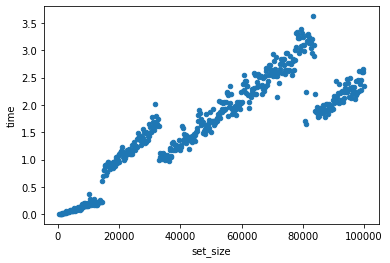
\includegraphics[width=0.95\textwidth]{bstree1.png}
    \caption{Time - Size(average)}
    \end{minipage}
    \begin{minipage}{0.5\textwidth}        
    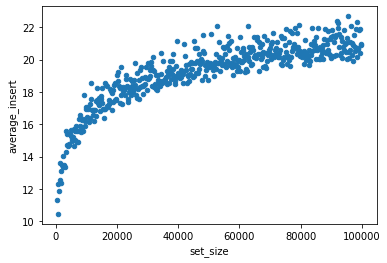
\includegraphics[width=0.95\textwidth]{bstree2.png}
    \caption{Average\_insert - Size(average)}
    \end{minipage}
    \begin{minipage}{0.5\textwidth}        
    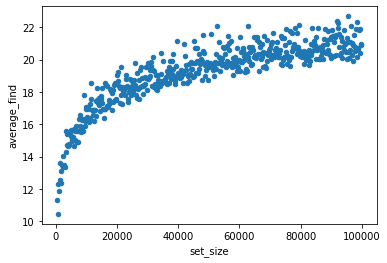
\includegraphics[width=0.95\textwidth]{bstree3.png}
    \caption{Average\_find - Size(average)}
    \end{minipage}
    \begin{minipage}{0.5\textwidth}
    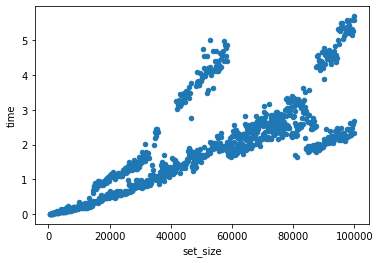
\includegraphics[width=0.95\textwidth]{bstree4.png}
    \caption{Time - Size(worst)}
    \end{minipage}
    \begin{minipage}{0.5\textwidth}        
    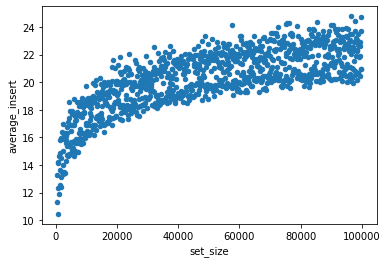
\includegraphics[width=0.95\textwidth]{bstree5.png}
    \caption{Average\_insert - Size(worst)}
    \end{minipage}
    \begin{minipage}{0.5\textwidth}        
    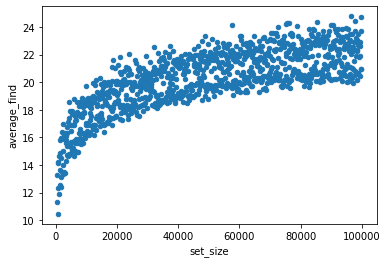
\includegraphics[width=0.95\textwidth]{bstree6.png}
    \caption{Average\_find - Size(worst)}
    \end{minipage}
\end{figure}
\noindent Average\_insert: the average number of data insertions.

\noindent Average\_find: the average number of data finds.

\subsection{Discussion}
When using linear probing, the relationship between dataset size and total time per operation, the average number of inserts and the average number of finds are shown in the six graphs above. First three are for average cases, and the rest are for worst cases.

From figure 5, it shows the relationship between time and size, with an overall trend of increasing time as size increases. It is worth noting that there are a few data that do not correspond to the overall trend when size were about 15000, 33000 and 80000. Due to the volume of data, deviations should be allowed.

From figure 6 and figure 7, they show the relationships between average insertions/finds and size. As the hashset size increases, the image trends for the average number of insertions/finds all follow the logn function trend, so the complexity of binary search tree in average cases should be O(logn).

From figure 8, it shows the relationship between time and size, with an overall trend of increasing time as size increases. It is worth noting that there are a few data that do not correspond to the overall trend when size were about 15000, 33000, 42000, 80000 and 90000. Due to the volume of data, deviations should be allowed.

From figure 9 and figure 10, they show the relationships between average insertions/finds and size. As the hashset size increases, the image trends for the average number of insertions/finds all follow the logn function trend, so the complexity of binary search tree in worst cases should be O(logn).

\subsection{Conclusion}
The hypothesis that the complexity of both the insertion and find operations will be O(logn) is satisfied in average cases, but in worst cases, the complexity should still be O(logn), which shows in the figures above.

\appendix

%% And raw data or code scripts you want to present should be included as appendices.

\end{document}


